\begin{figure}[H]
\centering
\begin{minipage}[t]{58mm}
\vspace{0pt}
\centering
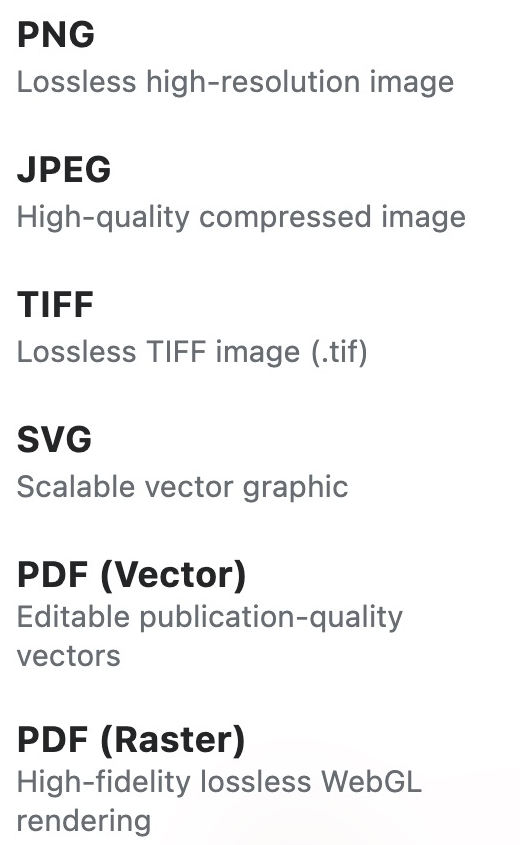
\includegraphics[width=52mm]{publication-assets/crop-496bc1fbfb3e99bfc4e7.png}
\end{minipage}\hspace{4mm}%
\begin{minipage}[t]{58mm}
\vspace{0pt}
{\centering
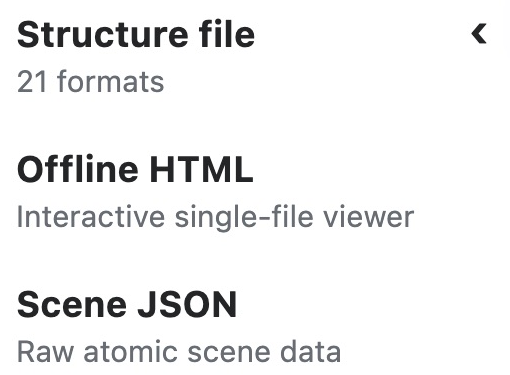
\includegraphics[width=51mm]{publication-assets/crop-68b4df9ea7d48ce9da1e.png}\par}
\par\vspace{3mm}
\raggedright\fontsize{9}{13}\selectfont
\ui{Structure file}保存所选格式能表达的模型信息。

\smallskip
\ui{Offline HTML}用于在本机浏览器中旋转观察。

\smallskip
\ui{Scene JSON}记录原子场景，区别于结构JSON。
\end{minipage}
\caption{原子查看器的两类导出菜单。左侧\ui{Export image}提供六种图像格式；右侧\ui{Export file}分别通向结构文件、离线页面与场景JSON。}
\label{fig:atomic-export-menus}
\end{figure}
